\subsection{Procedurální generace mapy}

\subsubsection{Prvotní pokus s generací za pomocí šachovnicového paternu}
Prvotním pokusem bylo vytvoření mapy za pomoci systému umísťování předem vytvořených prefabů v šachovnicovém paternu. Tento systém se dá kupříkladu velice efektině využít ve tvorbě některých 2D map. V tomto případě systém sice fungoval, ale byl velice omezený. Mapa působila nesoudržně a nebyla píliš přehledná. Z tohoto důvodu byl tento systém nahrazen a začala práce na mnohem komplexnějším systému, který na teoretické rovině nabízel mnoho výhod a velikou flexibilitu. Velmi raná verze mapy vytvořená pomocí šachovnicového systému je na obrázku \ref{fig:mapa_sachovnice}. Nový systém generace je popsán v kapitole níž v sekci \ref{sec:proceduralni_generace_mapy}.

\begin{figure}[ht]
    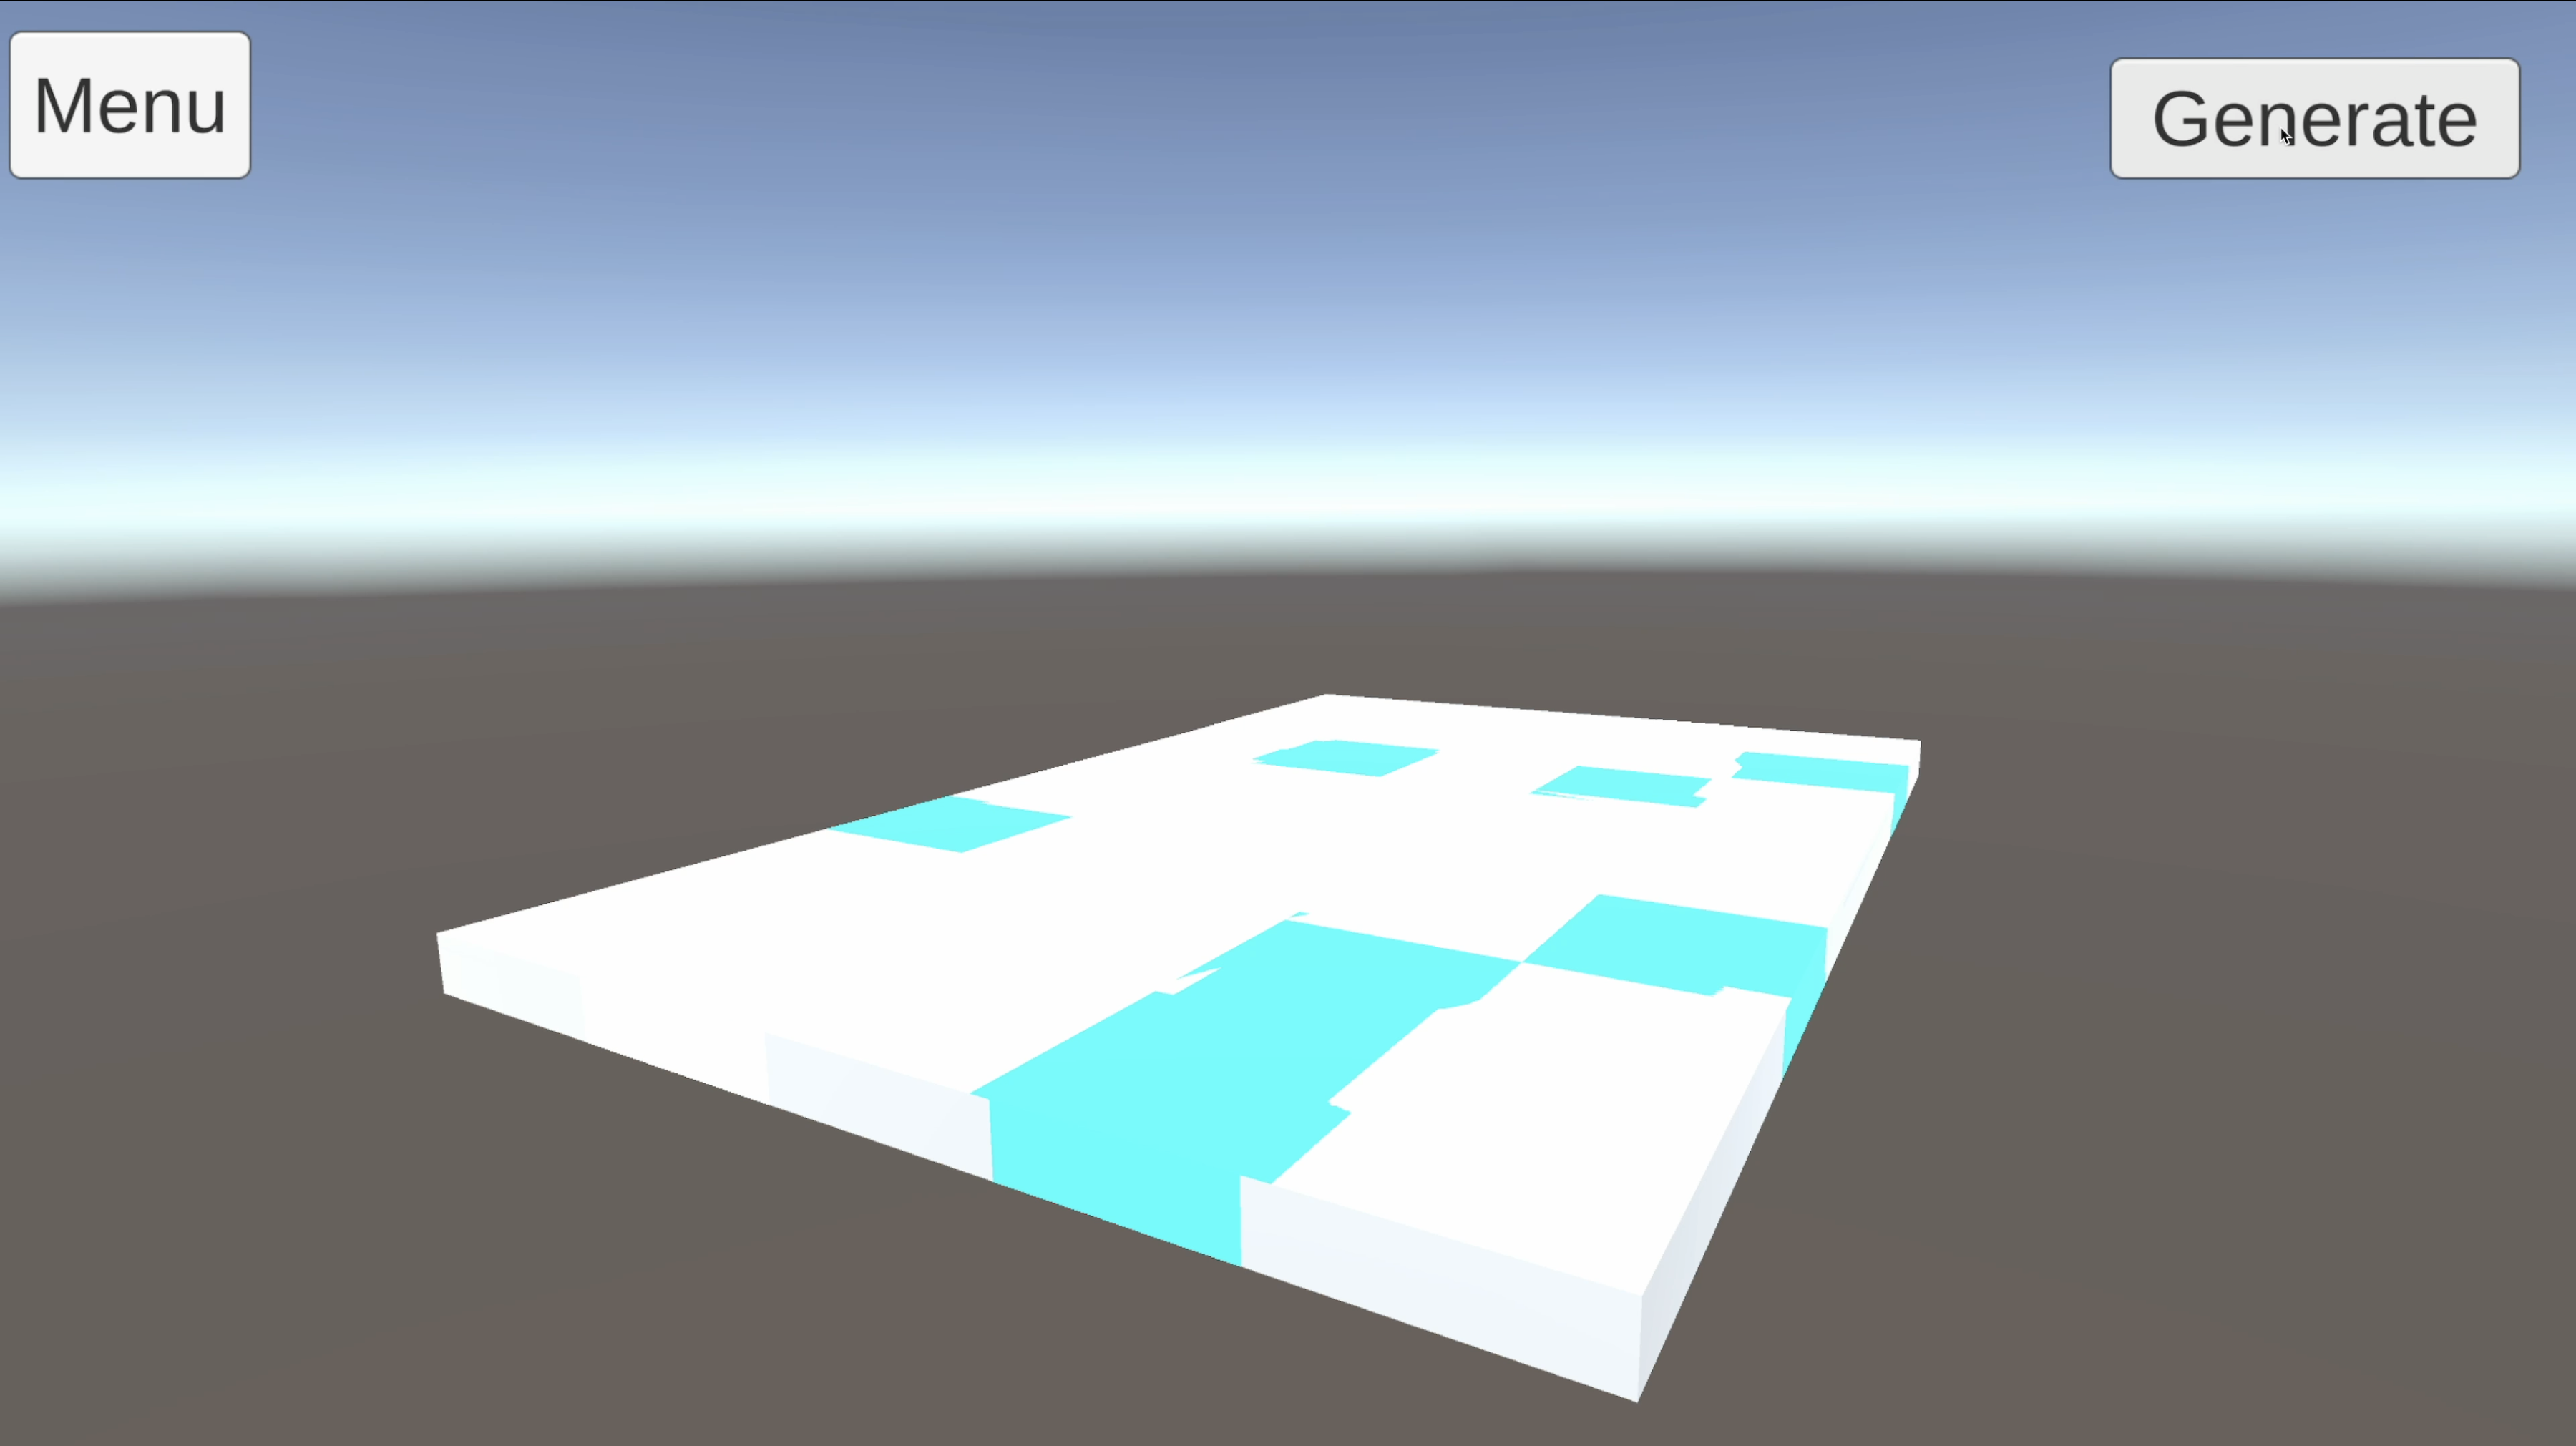
\includegraphics[width=\columnwidth]{mapa_sachovnice.png}
    \centering
    \caption{Raná verze mapy vytvořená pomocí šachovnicového systému}
    \label{fig:mapa_sachovnice}
\end{figure}

\subsubsection{Procedurální generace s náhodnými parametry}
\label{sec:proceduralni_generace_mapy}

Druhým pokusem bylo vytvoření mapy za pomoci procedurální generace s náhodnými parametry. Tento systém by nabízel velkou flexibilitu a mnoho možností.

Systém fungoval na principu náhodného výběru vstupních parametrů v limitních mezích. Tyto parametry rozhodly o velikosti první z místností. Následně byly vytvořeny další místnosti, které byly umístěny v okolí první místnosti tak, aby na ni přímo navazovaly, ale nepřekrývaly ji. Bylo zapotřebí využít délky a šířky první místnosti, vygenerovat délku a šířku místnosti druhé a v závisloti na hodnotách posunout pivotní bod základny druhé místosti na správné místo v 3D prostoru tak, aby místnosti navazovaly. Následně byla vygenerována další místnost a tak dále.

Poté došlo k vytvoření stěn o pevně dané šířce na hranách podstav místností. Délky těchto stěn přímo odpovídaly délkám a šířkám místností. Střed stěny byl umístěn v polovině délky podstavy od středu v odpovídající výšce.

Dalším prvkem bylo určení druhu místnosti. Bylo vytvořeno několik kategorií místností: kancelář, místnost nadřízeného, konferenční místnost, chodba, odpočívárna a sklad. Tyto kategorie byly následně přiděleny každé místnosti v závislosti na jejích parametrech. Podmínkou bylo, že některé místosti musí být obsaženy z důvodu průběhu hry. Pokud by kupříkladu nebyla přítomna kancelář, tak by chyběly potřebné počítačové stanice. Dalším příkladem je místnost nadřízeného, která musí obsahovat počítačovou stanici. Proto byly tyto kritické kategorie přiděleny v úvodu a to největší a nejmenší z místností. Dále byly zohledněny rozměry místností a jejich pozice na mapě. Například pokud byla místnost podlouhlá, tak se jednalo o chodbu. Zbytek místností byl přiřazen ze zbytku kategorií náhodně.

Tento systém byl velmi flexibilní a nabízel velké množství možností. Bohužel se nepodařilo jeho dokončení. Problém nastal při umísťování prefabů v prostoru. K umístění došlo, ale postup byl neefektivní a výsledek byl nesystematický. Proto byl tento systém nahrazen za systém, který je popsán v následující kapitole. Stále ale věřím, že se jedná o nejvíce zajímavý a flexibilní systém, u kterého není možné vyloučit jeho použití v budoucnu.

\subsubsection{Finální provedení}
\label{sec:finalni_provedeni_mapy}

Výsledné řešení je ve svém provedení částečně jednodušší než řešení popsané v předchozí kapitole. Výsledek je však dostatčný pro tvorbu iluze mnoha kombinací a opakujícího se prostředí mapy.

Generace funguje na principu umísťování prefabů do náhodných pozic z předem známého pole bodů v trojrozměrném prostoru. Mapa je prakticky statická a dochází tedy převážně ke změně pozic prefabů.

V prvním kroku je definováno pole pozic, které obsahuje několik možných pozic, na kterých lze umístit objekty. Poté je vytvořena funkce, která náhodně vybírá několik pozic z pole a na tyto pozice umísťuje náhodně vybrané objekty. Pro každý typ objektu je tento proces samostaný a proběhne tedy několikrát.

V kroku druhém jsou na mapy doplněny dodatečné objekty v závislosti na zabraných pozicích.

Tento systém je v dosavadní alfa verzi dostačující, ale jak již bylo zmíněno výše, je možné v budoucnu obnovit původní myšlenku procedurální generace, která by umožnila vytvořit více možností a vytvořit tak více dynamické prostředí.

\begin{figure}[ht]
    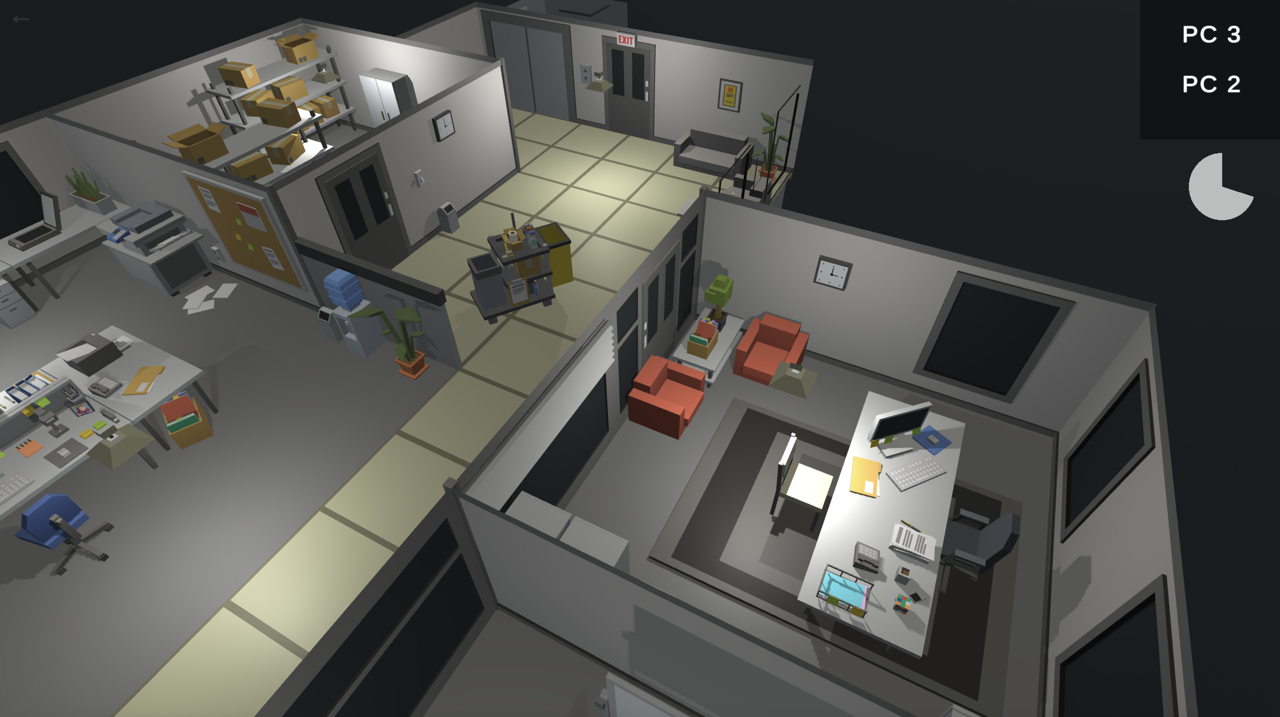
\includegraphics[width=\columnwidth]{mapa0.png}
    \centering
    \caption{Herní mapa kancelářského komplexu}
    \label{fig:mapa0_img}
\end{figure}
